\section{Attack Design}\label{sec:design}


The workflow of the {\attackName} attack in {\systemName} is shown in Figure~\ref{fig:flow}. The system can be separated into two parts: the user side and the attacker side. 
%
On the user side, a smartphone user downloads a seemingly harmless application and installs it on her device. Then the disguised app runs in the background and keeps monitoring the motion sensors. The sensor readings are then uploaded and sent to the attacker. 
%
On the attacker side, there are training steps and prediction steps. The training steps start from a training dataset that contains both sound data and motion data, while the input for prediction steps only contains motion data. 

The training steps first apply compressed sensing techniques on the sound data and build a learned dictionary from audio files, then process the corresponding motion data to remove unwanted signal components. With the preprocessed motion data and a learned dictionary,  the signal is reconstructed to a signal with more samples. Afterward, the reconstructed signal is fed to a Bidirectional Long Short-Term Memory (Bi-LSTM) network to train a classification model. 
The classification labels/classes (e.g. digits, genders, activity types, and so on) is determined by the sound data only.


\begin{landscape}
\begin{figure*}[h]
	\centering
	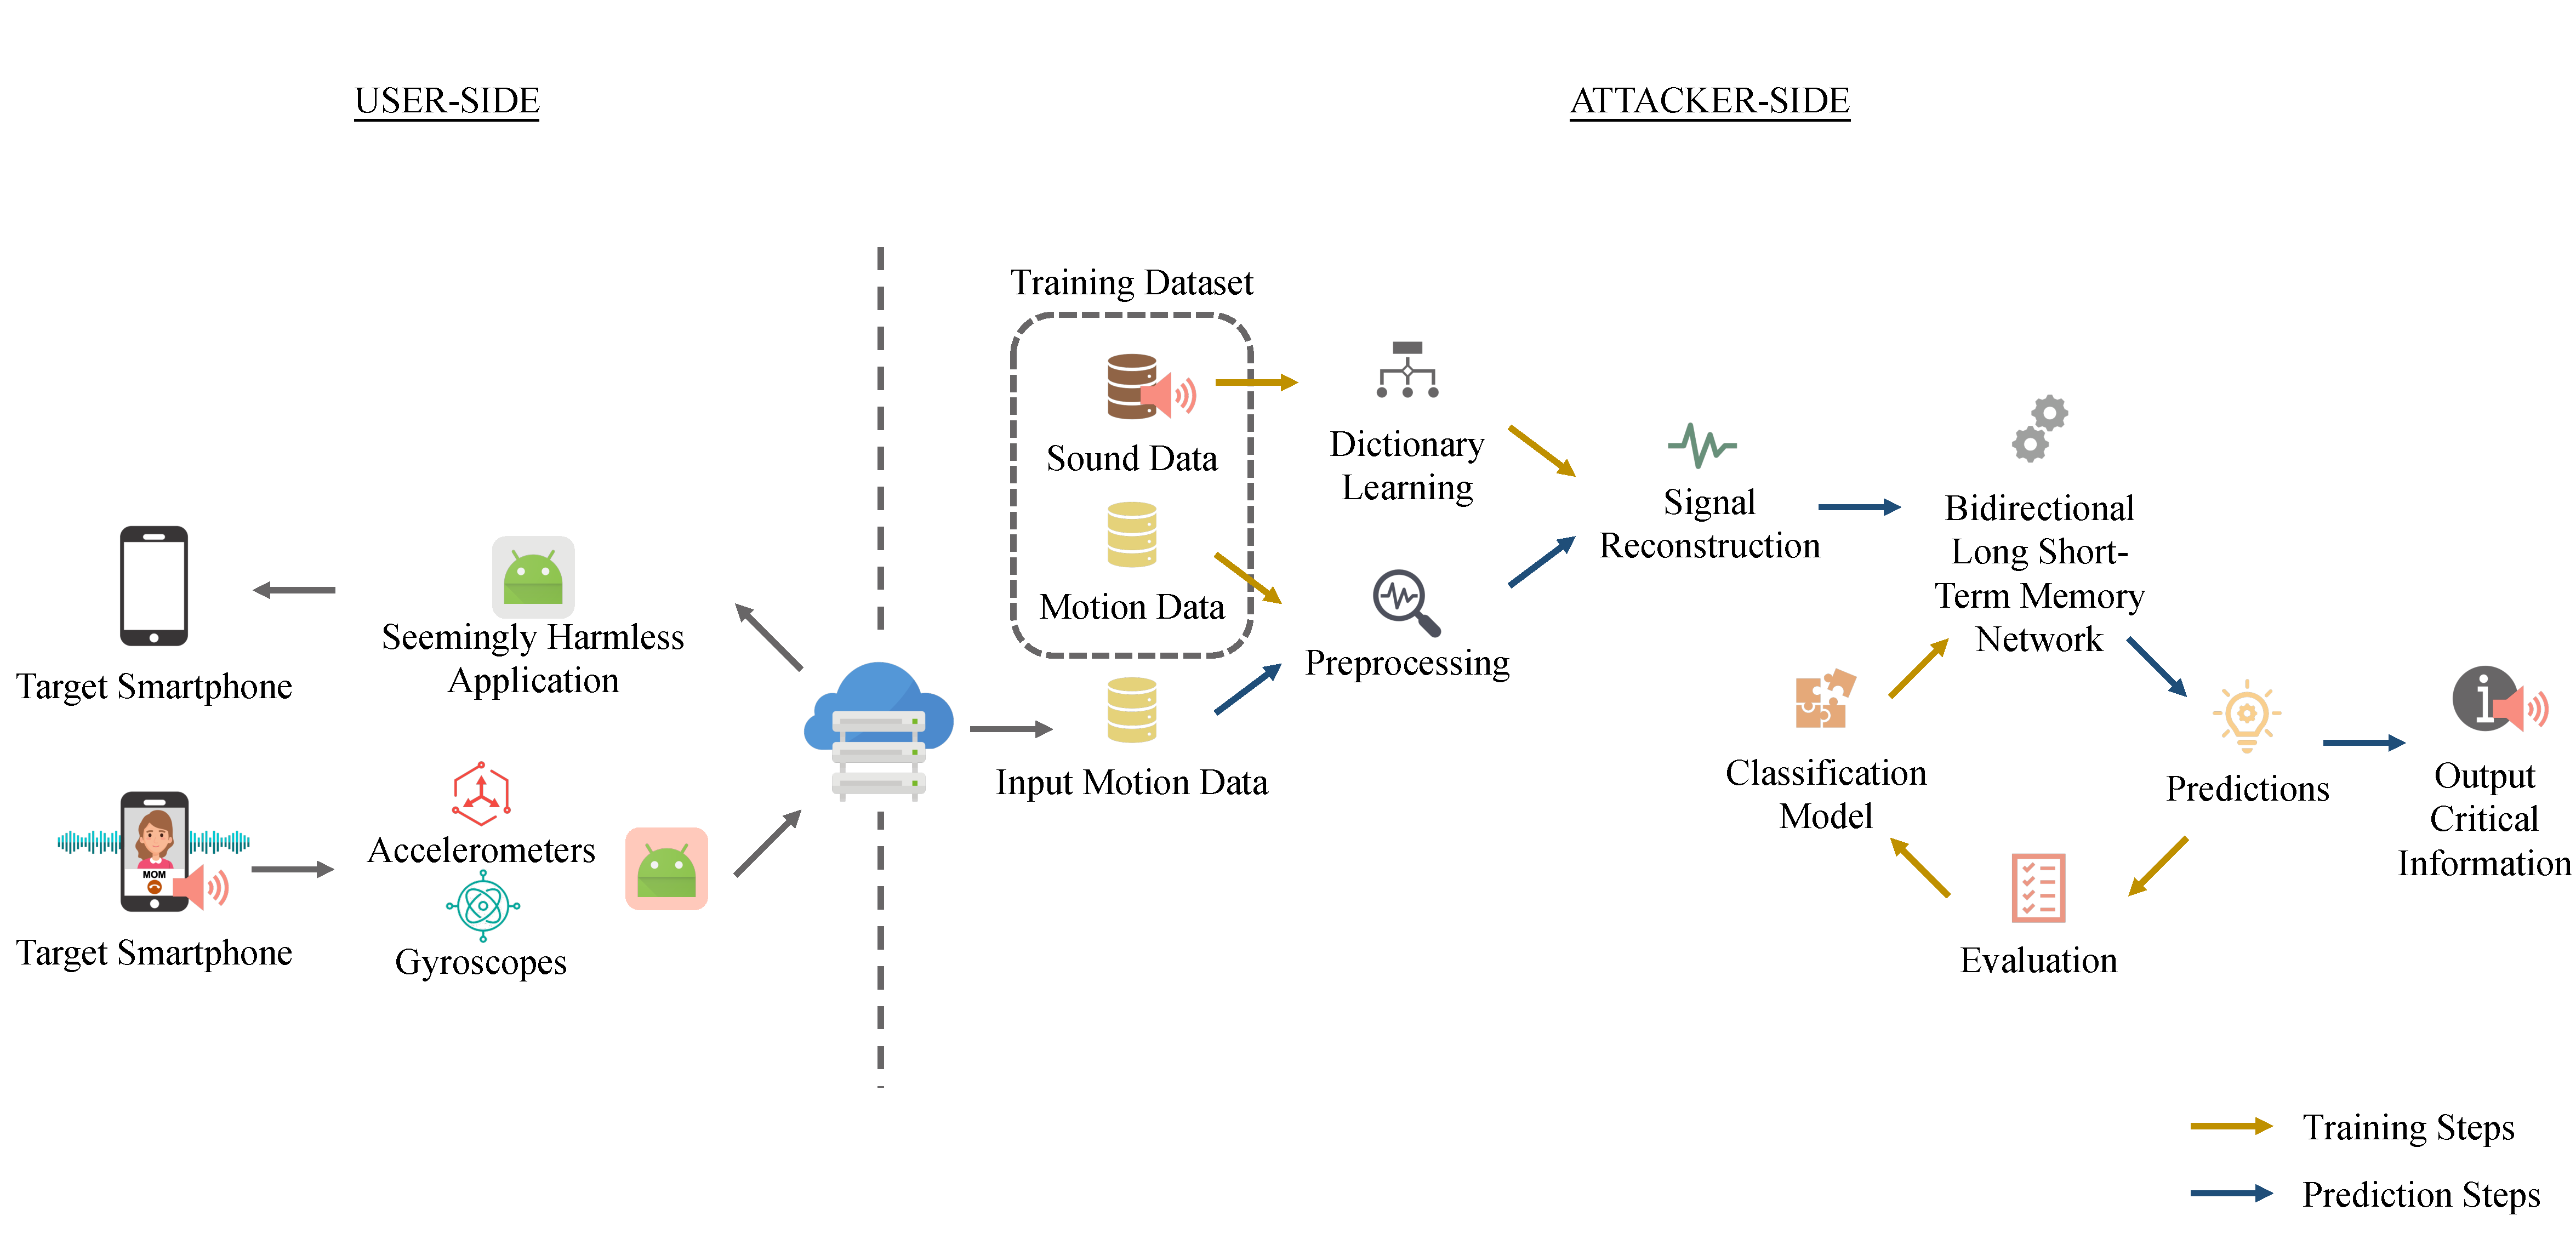
\includegraphics[width=\linewidth]{attackflow}
	\caption{The {\attackName} Attack Workflow in the {\systemName} System. }
	\label{fig:flow}
	%		\vspace{-.2in}
\end{figure*}
\end{landscape}



The prediction steps start with motion data, go by preprocessing, adopt the learned dictionary to reconstruct signals, and finally use the trained Bi-LSTM model to output critical information, without the presence of sound data.



In this section, we explain in detail how the {\systemName} system implements the {\attackName} attack to eavesdrop on digits played by smartphone speakers. A similar approach can be applied to obtain user activity type or speaker gender/identity as evaluated in Section~\ref{sec:experiment}.


\subsection{Training Dataset}

\begin{table}[h]
	\caption{Dataset Information}
	%	\footnote{Some part of the data is from~\cite{matyunin2018zero}, others are tested }
	\label{tab:dataset}
	\centering
	%	\resizebox{\columnwidth}{!}{
	\begin{tabular}{lcc} %{lp{2cm}p{2cm}}
		\toprule		
		%			\multirow{2}{3cm}{Dataset}
		%			& TIDIGITS & Speech Commands\\
		%			& \cite{leonard1993tidigits} & \cite{warden2018speech}\\
		%			
		Dataset & TIDIGITS~\cite{leonard1993tidigits} & Speech Commands~\cite{warden2018speech}\\
		\midrule
		Sampling Rate & 20,000 Hz & 16,000 Hz\\
		No. Speakers & 326 & 2,618\\
		Labels & 11 Digits & 35 Command Words \\
		No. Utterances & 7,172& 105,829\\
		Training Size & 3,586 & 84,843\\
		Validation Size & - & 9,981\\
		Testing Size & 3,586 & 11,005\\
		\bottomrule
	\end{tabular}
	%}
\end{table}

As shown in Table~\ref{tab:dataset}, we use two datasets, TIDIGITS and Speech Commands. 

TIDIGITS~\cite{leonard1993tidigits} are professional recordings of isolated digits, which has been used in~\cite{michalevsky2014gyrophone} and \cite{anand2019spearphone}. Therefore, in the main sessions of this chapter, we illustrated our system using this dataset for the comparison's purpose. However, TIDIGITS only contains digits, and the utterances are all recorded in laboratory conditions. It is natural that the accuracy would be higher on such a dataset. Therefore, we consider another dataset Speech Commands~\cite{warden2018speech}, which is the TensorFlow Speech Commands Dataset(Version 2). This dataset can be used for limited-vocabulary speech recognition. It consists of 105,829 utterances of 35 command words such as up, down, forward, stop, house, happy, etc. This dataset is recorded by a web-based application in a crowd-sourcing manner. Speakers are from all over the world and they speak the commands in uncontrolled environments. Basically, if a model trained on Speech Commands works well, it indicates that any piece of speech recordings online can be used as the training data for the {\systemName} system. The result using this dataset is shown in Section~\ref{sec:word}, the correct rate is 83.2\%.



From now on, we focus on TIDIGITS.


\begin{figure}[H]
	\centering
	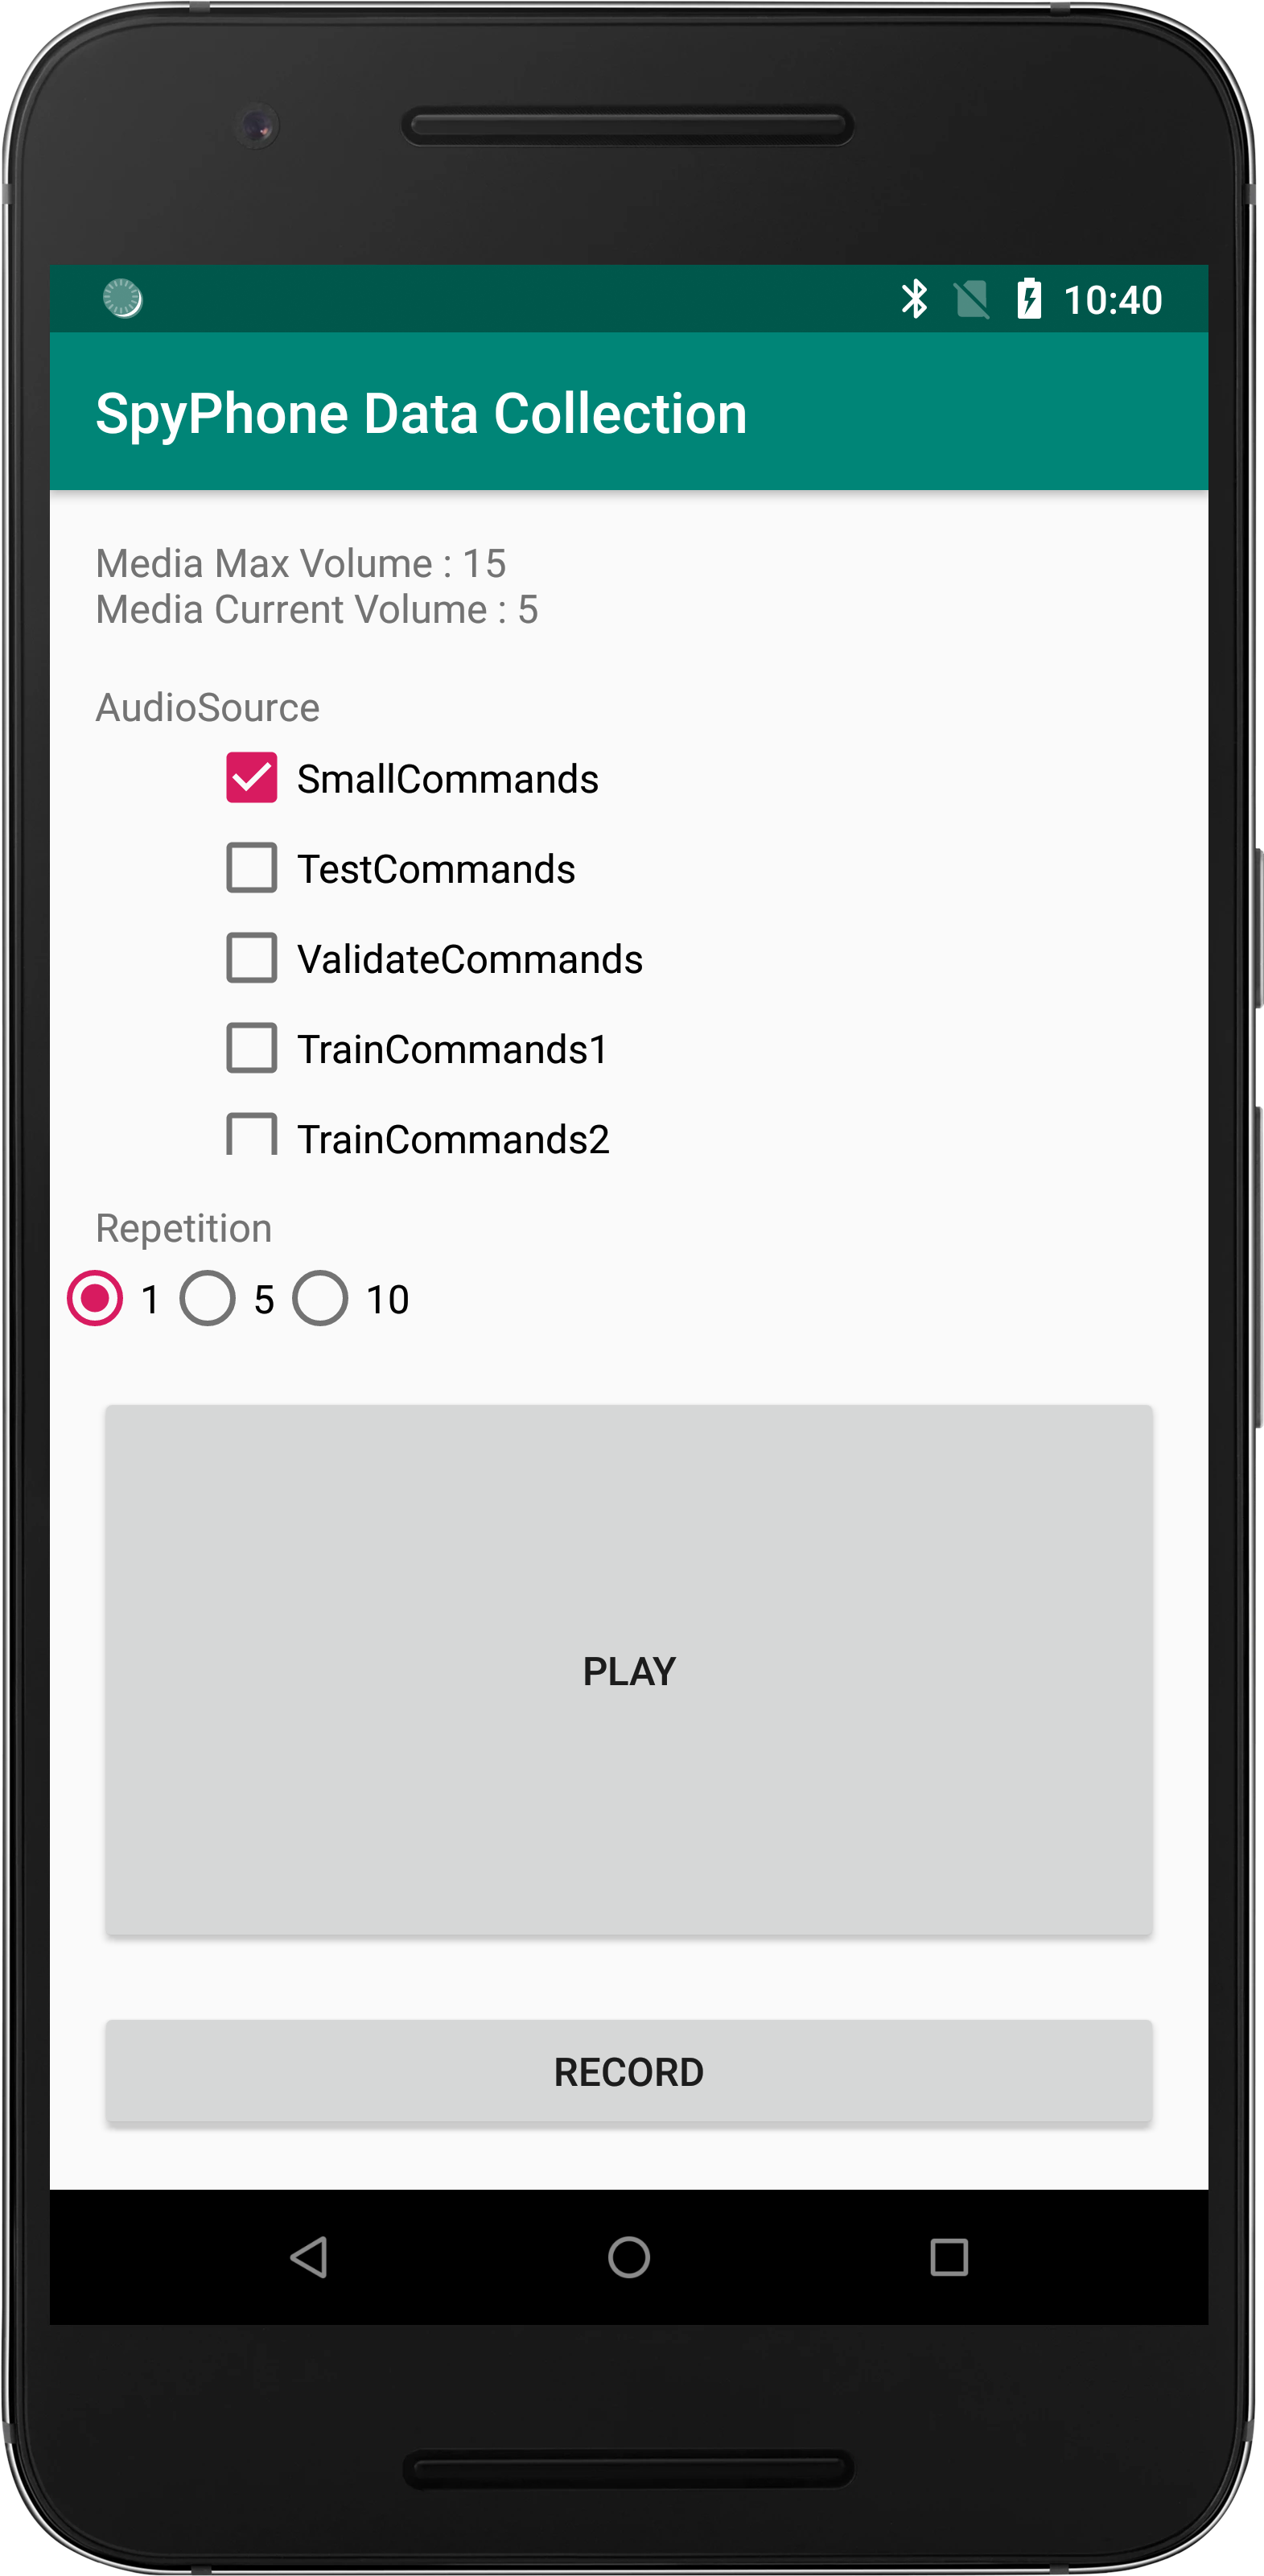
\includegraphics[height=.4\textheight]{SpyPhoneData}
	\caption{{\spp} Data Collection Application}
	\label{fig:spyphoneapp}
\end{figure}

In the beginning, the TIDIGITS dataset is used to build both the sound data and the motion data for the training dataset.
%
This corpus contains speech of 11 isolated digits: ``one'', ``two'', \ldots, ``nine'', ``zero'' and ``oh'', which are collected using an Electro-Voice RE-16 Dynamic Cardiod microphone, digitized at 20,000 Hz.
%
These audio files are directly used as training sound data. 
The motion data, however, are collected by playing these audio files using the built-in speakers of a Google Nexus 6P device. They are the simultaneous recordings from the same phone's  accelerometers and gyroscopes with a sampling rate of 400 Hz.
When playing the sound, the volume is set to be the highest level since these data will be used for training and the higher volume, the higher accuracy (according to experiments in Section~\ref{sec:impact:volume}).
Note that when the {\attackName} attack is conducted in practice, the input motion data may come from a lower volume setting defined by the user. The attacker cannot control the volume setting of the target smartphone, but she can control the volume when building the training dataset. 
%
For the training dataset, only part of the sound and motion data are used. The impact of the training data size on the prediction accuracy is elaborated in Section~\ref{sec:impact:trainsize}.
All data are collected by the SpyPhoneApp as shown in Figure~\ref{fig:spyphoneapp}.



 \begin{algorithm}[!t]
	\small
	\DontPrintSemicolon
	\LinesNumbered
	\SetKw{KwRead}{audioRead}
	\SetKw{KwRemove}{removeSilence}
	\SetKw{KwKVSD}{kvsd}
	\SetKw{KwShift}{shiftLeft}
	\SetKw{KwDown}{downSample}
	\SetKw{KwBuffer}{buffer}
	\SetKw{KwConca}{concatenate}
	\KwIn{Training Sound Dataset $\mathcal{T}_i$ for class $i$, Downsample Rate $r$, Dictionary Size $(N, K)$ }
	\KwOut{Dictionary $D_i$ for class $i$}
	$ S_i \leftarrow []$ \tcp*{Initialize training vectors} 
	\ForEach{audio file $\tau$ in $\mathcal{T}_i$}{
		\tcp{get signal $s$ and sampling frequency $fs$}
		$[s, fs] = \KwRead(\tau)$\;  
		\tcp{remove unvoiced part}
		$s\leftarrow  \KwRemove(s)$\;
		\tcp{downsample signal to $r$ subsignals and buffer each subsignal of length $N$}
		\ForEach{$j$ from 1 to $r$}{
			$s \leftarrow \KwShift(s, 1)$  \tcp*{shift left by 1 sample}  \label{line:shift}
			$ss \leftarrow \KwDown(s, r)$\; \label{line:down}
			$bs \leftarrow \KwBuffer(ss, N)$  \;
			$S_i \leftarrow \KwConca(S_i, bs)$
			
		}
		
	}
	\tcp{run K-SVD dictionary training algorithm}
	$D_i \leftarrow \KwKVSD(S_i, N, K)$
	\caption{{BuildDictionary}\label{algo:builddic}}
\end{algorithm}

\subsection{Dictionary Learning}\label{sec:design:dict}

\begin{figure*}[ht]
	\centering
	\includegraphics[width=.55\linewidth]{dict}
	\caption{Example of Learned Dictionary Atoms. For each digit class, two different atoms are shown.}\label{fig:atoms}
\end{figure*}

We now demonstrate how to construct efficient representations of audio files by building a dictionary learned from the data itself. 
Recall Section~\ref{sec:compressed}, a learned dictionary is used to reconstruct a signal when it is undersampled. 
%
In the {\systemName} system, the sound data are the signals of interest while the motion data are the measurements. The training sound data are grouped into 11 classes, (one to nine, zero, and oh). For each class $i$, the dataset is denoted by $\mathcal{T}_i$ and the representation dictionary $D_i$ is computed by Algorithm~\ref{algo:builddic}.

As shown in Figure~\ref{fig:compressed}, each representation dictionary $D_i$ is a collection of $K$ atoms, where each atom is a column vector of length $N$. An atom is basically some typical patterns of the signal of interest. For sound signal $s_i$ of class $i$,
it should be represented or approximated as a linear combination of some few of the dictionary atoms. Mathematically,
%\begin{displaymath}
	$s_i = D_i * w_i,$
%\end{displaymath} 
for each column $s_i$ in $S_i$. Here $S_i$ is the training vectors calculated in Algorithm~\ref{algo:builddic}. Compared to the original sound signal from an audio file, $S_i$ is the result from many functions including \verb|removeSilence()|, \verb|downSample()|, and \verb|buffer()|. 
 
 
 
Note that the length of a dictionary atom must be the same as the length of the training vector $s_i$. Since the original sound signal can have at most 2 s $\times$ 20,000 Hz = 40,000 samples (The duration of audio files in the dataset is at most 2 seconds.). If directly using original sound to train the dictionary, the atom size must be 40,000 as well. However, not all signals in an audio file are informative. By applying \verb|removeSilence()|, the unvoiced part of the audio signals is removed, which significantly improves the space and time efficiency of the algorithm. The \verb|removeSilence()| is based on \cite{rabiner2011theory}, which calculates the short-time energy of signals and conducts zero-crossing analysis to differentiate sounding and unvoiced parts.
 
 

Moreover, from voice acoustics elaborated in Section~\ref{sec:voice}, the most informative frequency range is roughly 100-4000~Hz, the 20,000~Hz sampling rate oversamples human speech. Therefore, to build a better representation dictionary, we shift the signals (Line~\ref{line:shift} in Algorithm~\ref{algo:builddic}) and downsample it (Line~\ref{line:down} in Algorithm~\ref{algo:builddic}) by keeping the first sample and then every $r$-th sample after the first. The impact of the downsample rate $r$ is evaluated in Section~\ref{sec:impact:downrate}.

Last but not least, different people say different digits with intrinsically different time duration, which results in different signal lengths. To build a general representation dictionary, we buffer every signal with the fixed buffer size as $N$ using \verb|buffer()|. In other words, no matter how long is the original sound signal, by Algorithm~\ref{algo:builddic}, it is transformed into a matrix $S_i$ with $N$ rows. The number of columns, however, is not fixed. For convenience's sake, we denote this number as $L_i$.




 
Dictionary Learning is the process of finding a dictionary, $D_i$ of size $N \times K$, and a corresponding coefficient matrix $W_i$ of size $K \times L_i$ such that the approximations of the training vectors, $S_i$ of size $N \times L_i$, are as good as possible, given a sparseness criterion on the coefficients. Mathematically, the dictionary learning problem can be formulated as an optimization problem with respect to $D_i$ and $W_i$:
%$
\begin{displaymath}
	\left\lbrace 
	D_{i, opt},
	W_{i, opt}
	\right\rbrace 
	=
	\argmin_{D_i, W_i}
	\sum_{l=1}^{L_i}
	\left( 
	\gamma
	\Vert w_{i, l} \Vert_p
	+
	\Vert s_{i,l} - D_i w_{i, l} \Vert_2
	\right) 
	,
%	$
\end{displaymath}
where $\gamma$ and $p$ are as in Eq.~(\ref{eq:reconstruction}), $s_{i, l}$ is the $l$-th column of $S_i$, and $w_{i, l}$ is the $l$-th column of $W_i$. 




The solver we use for this optimization problem is K-SVD~\cite{aharon2006k}, as it is one of the most well-known shared dictionary learning algorithms~\cite{xu2017survey}. We did not test all existing dictionary learning algorithms, but among those we tested, PCA~\cite{haykin2007neural}, K-SVD,  and GAD~\cite{jafari2011fast}, K-SVD provides the best results. 




K-SVD is an iterative method with two main steps: First, keep $D_i$ fixed then solve $W_i$, which is essentially $L_i$ separate problems as in Eq.~(\ref{eq:reconstruction}); Second, keep only non-zero positions in $W_i$ fixed and find $D_i$ and $W$ using singular-value decompositions (SVD). Figure~\ref{fig:atoms} shows the first two atoms in the learned dictionary of each digit class using K-SVD. Generally, the atoms are different inter-class and similar intra-class.

By concatenating every $D_i$ together, the overall dictionary is 
\begin{equation}
	D = \left[ D_1, D_2, \ldots, D_i, \ldots, D_{11} \right], \label{eq:dictConcat}
\end{equation}
which will be used for signal reconstruction in later steps.





\subsection{Motion Data Preprocessing}
The input motion data are collected similarly to how motion data are collected for the training dataset, i.e., playing TIDIGITS audio files by the smartphone's built-in speakers. However, since these data are to simulate the attacking scenarios in reality, the data are collected multiple times using 15 different volume settings (Section~\ref{sec:impact:volume}). Moreover, we collected the motion data in both quiet and noisy environment (Section~\ref{sec:impact:noise}), and in both stable and moving states (Section~\ref{sec:impact:move}).
\begin{figure*}[!h]
	\centering
	\includegraphics[width=.8\linewidth]{preprocess0}
	\caption{The Magnitude and Phase Response of the FIR Highpass filter.}\label{fig:spyphoneresponse}
\end{figure*}


\begin{figure}[H]
	\begin{minipage}[t]{.45\linewidth}
		\centering
		\includegraphics[width=\linewidth]{preprocess1}
		\includegraphics[width=\linewidth]{preprocess2}
		\vspace{-.2in}
		\subcaption{Raw Motion Data.}\label{fig:rawmotion}
		\vspace{.2in}
		\includegraphics[width=\linewidth]{preprocess3}
		\vspace{-.2in}
		\subcaption{Spectrogram of Raw Motion Signals.}\label{fig:rawspec}
	\end{minipage}
	\begin{minipage}[t]{.05\linewidth}
		\quad
	\end{minipage}
	%\end{figure}
	%
	%\begin{figure}\ContinuedFloat	
	\begin{minipage}[t]{.45\linewidth}
		\centering
		\includegraphics[width=\linewidth]{preprocess4}
		\vspace{-.2in}
		\subcaption{Spectrogram of Proceseed Signals.}\label{fig:newspec}
		\vspace{.2in}
		\includegraphics[width=\linewidth]{preprocess5}
		\includegraphics[width=\linewidth]{preprocess6}
		\vspace{-.2in}
		\subcaption{Preprocessed Motion Data}\label{fig:newmotion}
	\end{minipage}
	
	\caption[Preprocessing of Motion Data. ]{Preprocessing of Motion Data. The top two figures show the raw data from 3-axis accelerometers and 3-axis gyroscopes. There are 450 samples shown in the figure. These samples span about one second (450 / 400Hz = 1.125s) and are collected when the user is dropping the head of the phone while playing a ``Zero'' utterance from a male speaker. The frequency of such movement is far less than the frequency of human voices. Therefore, by applying the high pass filter, the noise caused by hand movements will be removed. }
	
	\label{fig:spyphonepreprocess}
\end{figure}

As mentioned in Section~\ref{sec:intro}, the motion data is impeded by low sampling rates, weak target signals, and large  interference  noises. To overcome such problems, we must preprocess the motion data. We apply a high pass filter to mitigate the noise and increase the signal-to-noise ratio. The cutoff frequency is set to be 50 Hz, since noises such as walking or other human body movements are unlikely to generate signals as high as 50 Hz.
We also use the speech-background separation algorithms from \cite{rabiner2011theory} to differentiate the data affected by sound signals from those do not. The red vertical lines in Figure~\ref{fig:rawmotion} are the borderlines between the speech part and the background part. 
Figure~\ref{fig:rawspec} and Figure~\ref{fig:newspec} show that various noises can be removed by applying a high pass filter.
The result after the preprocessing stage is shown in Figure~\ref{fig:newmotion}. These data will be used in the next signal reconstruction stage.



\subsection{Signal Reconstruction}
In this stage, the preprocessed motion data will be used to reconstruct the original audio data.

Mathematically, the goal of signal reconstruction is to solve $w^\prime$ in 
%$$$$ 
%\vspace{-.2in}
%\begin{displaymath}
	$x = R \times w^\prime$
%\end{displaymath}
as in Figure~\ref{fig:compressed}. Here the measurement $x$ is the motion data after preprocessing, and the reconstruction matrix $R$ is calculated by
\begin{equation}
R = S \times D, \label{eq:reconstruct2}
\end{equation}
where $S$ is the sensing matrix and $D$ is the dictionary obtained in Section~\ref{sec:design:dict}.

In the {\systemName} system, the sensing matrix describes the sensing procedure from audio data to motion data, which can be regarded as a downsampling operation. The downsampling rate ($r$) is determined by the sampling frequencies of smartphone speakers ($f_1$) and motion sensors ($f_2$): $r = f_1/f_2$. For example, a sensing matrix with downsample rate $r=3$ is as follows:
\begin{displaymath}
\small
S = 
\begin{bmatrix} 
1 & 0 & 0 & 0 & 0 & 0 & 0 & \cdots & 0  & 0& 0\\
0 & 0 & 0 & 1 & 0 & 0 & 0 & \cdots & 0 & 0& 0\\
0 & 0 & 0 & 0 & 0 & 0 & 1 & \cdots & 0 & 0& 0\\
\vdots & \vdots & \vdots & \vdots & \vdots & \vdots & \vdots &  & \vdots & \vdots & \vdots\\
0 & 0 & 0 & 0 & 0 & 0 & 0 & \cdots & 1 & 0& 0\\       
\end{bmatrix}.
\end{displaymath}
%
In the {\systemName} system, the true value of this rate can be as high as 48,000~/~ 400~ = 120, which indicates a huge information loss and a big challenge to recover the signals.
%
Note that Algorithm~\ref{algo:builddic} also has a downsampling operation (Line~\ref{line:down}), therefore the $R=S \times D$ operation can be replaced by changing the parameter $r$ in Algorithm~\ref{algo:builddic}. When reconstructing the signals, $D$ is used as $R$. The impact of the downsample rate $r$ is evaluated in Section~\ref{sec:impact:downrate}.
%
To solve Eq.~(\ref{eq:reconstruct2}), GPSR~\cite{figueiredo2007gradient} is used, which is able to find  
$
%\begin{displaymath}
w^\prime_{opt}
=
\argmin_{w^\prime}
\left( 
\gamma
\Vert w^\prime \Vert_p
+
\Vert x - R w^\prime \Vert_2
\right)
. 
$
%\end{displaymath}
The last step is to reconstruct the signal of interests by
$
%\begin{displaymath}
s^\prime = D \times w^\prime_{opt}.
%\end{displaymath}
$
These signals will be used as training data for the Bi-LSTM network discussed in the next section.




\begin{figure}[!b]
	\centering
	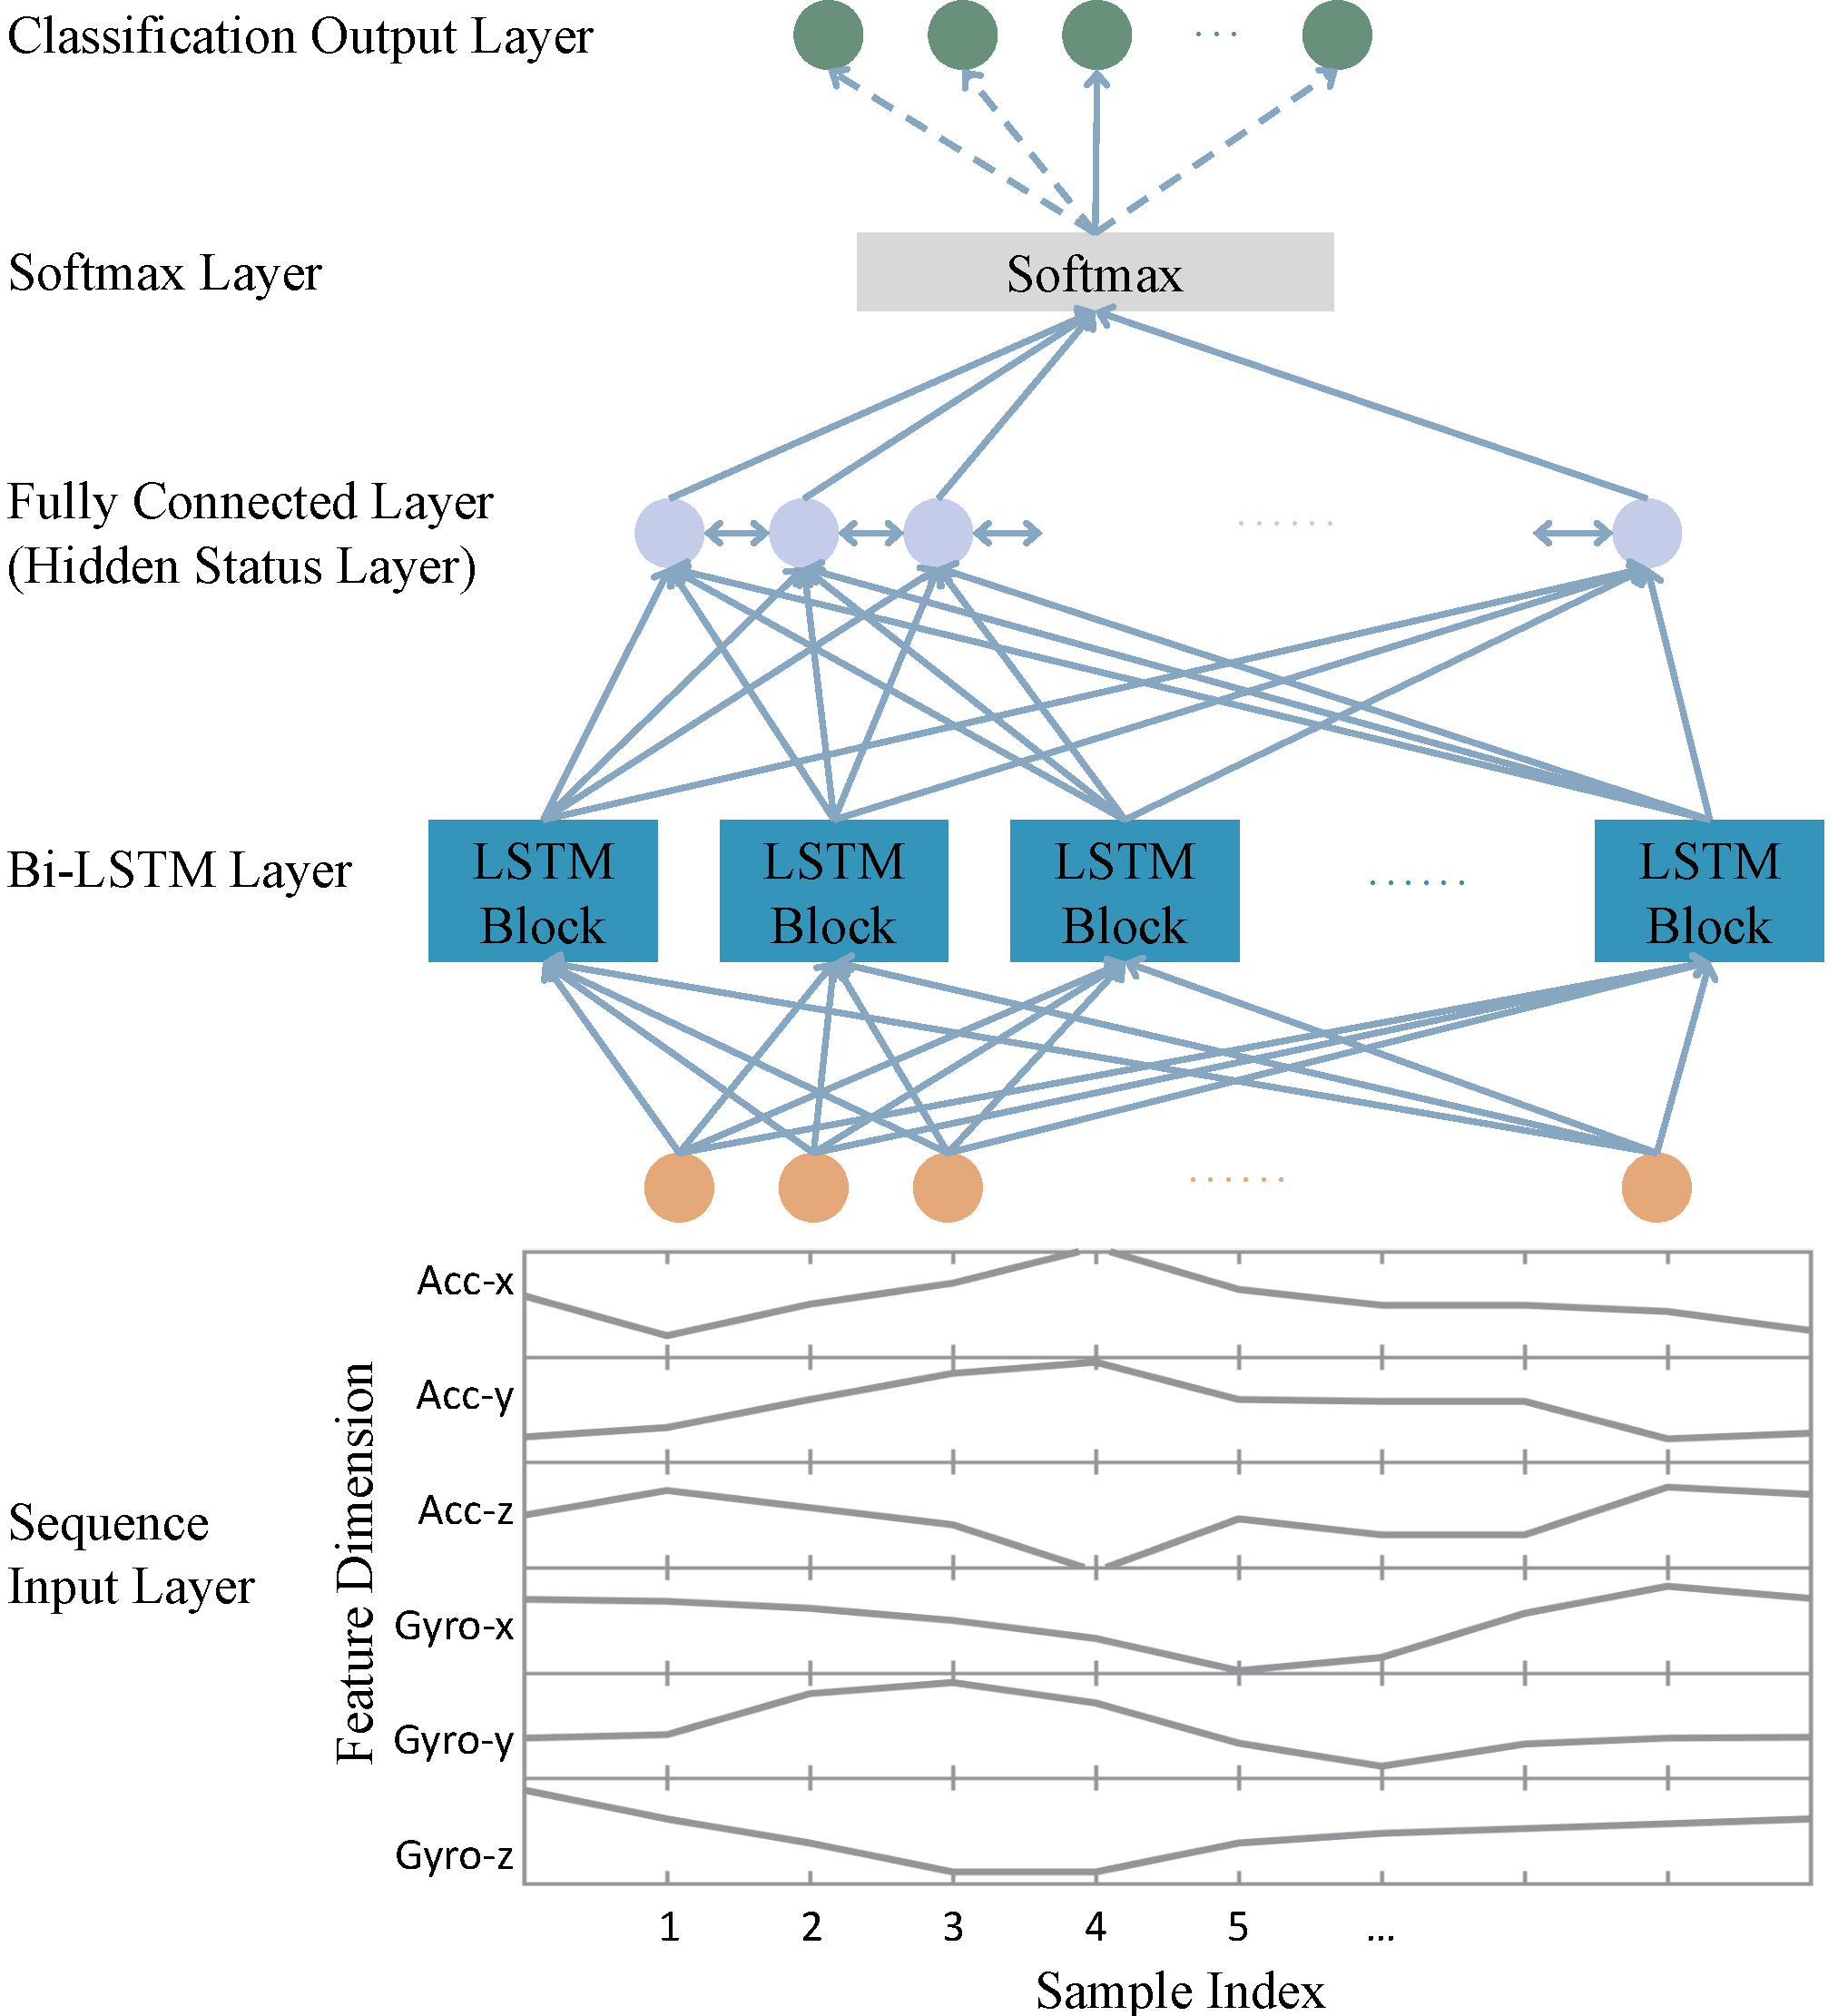
\includegraphics[width=.65\linewidth]{rnn}
	\caption{The Bidirectional Long Short-Term Memory Network (Bi-LSTM Network).}
	\label{fig:rnn}
\end{figure}


\subsection{Bi-LSTM Learing}\label{sec:LSTM}

The last stage is to use the reconstructed data to establish a Bi-directional Long Short-Term Memory (Bi-LSTM) network model, which will be used for classifying the input data later on.
%
 LSTM was first proposed by Sepp Hochreiter and J{\"u}rgen Schmidhuber in 1997 ~\cite{hochreiter1997long}. It is a special variant of  Recurrent Neural Networks (RNN), and is widely used in learning, processing, and classifying \textit{sequential } data because of 
its great property of selectively remembering patterns for long durations of time. 
%
Over the years, there have also been many variants of LSTM networks. However, based on a study in 2017, none of the variants can improve upon the standard LSTM architecture significantly~\cite{greff2017lstm}. Therefore, we still choose to implement the standard LSTM network in this work except for the bi-directional calculation. The original unidirectional LSTM network only preserves information from the inputs seen in the past. Bi-LSTM network, on the contrary, preserves information both from the past and the future. 
%
As shown in Figure~\ref{fig:rnn}, our Bi-LSTM network has five layers in total. In the sequence input layer, the input data have 6 feature dimensions, which consists of 3 accelerometer dimensions and 3 gyroscope dimensions. Then we establish an LSTM layer formed by LSTM blocks, where each block publishes its cell state to the next LSTM block. The output of the LSTM layer is sent to the fully connected hidden status layer. We set the total number of hidden units to be 100, and each hidden unit has two hidden states, one from the past and the other from the future. Then we feed the combined hidden status to a softmax function and output the classification results.





